
\documentclass[12pt,openright,oneside,a4paper,english,brazil]{abntex2}

\usepackage{graphicx}

\newcommand{\cabecalhoinstitucional}{
    \begin{minipage}[t]{0.20\textwidth}
        
\includegraphics[width=\linewidth]{logo-puc.png}
    \end{minipage}
    \hfill
    \begin{minipage}[t]{0.7\textwidth}
        \raggedright%
        {\ABNTEXchapterfont\large \textbf{PONTIFÍCIA UNIVERSIDADE CATÓLICA DO PARANÁ}}\\[0.3cm]
        {\large PRÓ-REITORIA DE PESQUISA, PÓS-GRADUAÇÃO E INOVAÇÃO}\\[0.3cm]
        {\large PROGRAMA DE INICIA\c{C}\~AO CIENT\'IFICA PARA ESTUDANTES DO ENSINO \`A DIST\^ANCIA -- PIC-EaD}\\
    \end{minipage}
}


\setlength{\parindent}{1.5cm}
\setlength{\parskip}{0.2cm}

\titulo{IMPLEMENTAÇÃO DE ALGORITMO DE SELEÇÃO INTELIGENTE DE ATRIBUTOS EM BASES DE DADOS MULTIMODAIS PARA PROBLEMAS DE INTELIGÊNCIA ARTIFICIAL NA INDÚSTRIA}
\autor{Gustavo Luiz de Jesus Zeloni}
\orientador{Prof (a). Wellington Rodrigo Monteiro}
\local{CURITIBA}
\data{2025}
\instituicao{%
  Pontifícia Universidade Católica do Paraná\\
  Pró-Reitoria de Pesquisa, Pós-Graduação e Inovação\\
  PROGRAMA DE INICIAÇÃO CIENTÍFICA PARA ESTUDANTES DO ENSINO À DISTÂNCIA -- PIC-EaD
}
\tipotrabalho{Relatório Final apresentado ao Programa Institucional de Bolsas de Iniciação Científica e Tecnológica da PUCPR}

\begin{document}

\begin{capa}
    \cabecalhoinstitucional%

    \vspace{2cm}

    \begin{center}
        {\ABNTEXchapterfont\bfseries\LARGE RELATÓRIO FINAL}\\[1.5cm]
        {\ABNTEXchapterfont\bfseries\Large IMPLEMENTAÇÃO DE ALGORITMO DE SELEÇÃO INTELIGENTE DE ATRIBUTOS EM BASES DE DADOS MULTIMODAIS PARA PROBLEMAS DE INTELIGÊNCIA ARTIFICIAL NA INDÚSTRIA}\\[2cm]
    \end{center}

    \vfill

    \begin{flushright}
        {\large Gustavo Luiz de Jesus Zeloni}\\
        {\large Wellington Rodrigo Monteiro}\\
        {\large Análise e Desenvolvimento de Sistemas - PUC-PR}\\
        {\large EAD}\\[2cm]
        {\large Curitiba}\\
        {\large 2025}
    \end{flushright}
\end{capa}

\newpage
\thispagestyle{empty}
\cabecalhoinstitucional

\vspace{2cm}

\begin{center}
    {\large Gustavo Luiz de Jesus Zeloni}\\[0.3cm]
    {\large Wellington Rodrigo Monteiro}\\[0.3cm]
    {\large Análise e Desenvolvimento de Sistemas - PUC-PR}\\[0.3cm]
    {\large Bolsista PUCPR}\\[3cm]

    \vspace{1.5cm}

    \begin{flushright}
    \begin{minipage}{0.55\textwidth} % ajuste aqui a largura
        \footnotesize % ou \scriptsize se quiser ainda menor
        Relatório Final apresentado ao Programa Institucional de Bolsas de Iniciação Científica e Tecnológica,\\
        Pró-Reitoria de Pesquisa, Pós-Graduação e Inovação da Pontifícia Universidade Católica do Paraná.\\[0.3cm]
        Orientador (a): Prof (a). Wellington Rodrigo Monteiro
    \end{minipage}
\end{flushright}

\vspace{2cm}

    {\large Curitiba}\\
    {\large 2025}
\end{center}

% Folha de rosto
\imprimirfolhaderosto

% Resumo
\begin{resumo}
Este relatório final apresenta a implementação e avaliação de um algoritmo de otimização multiobjetivo, especificamente o NSGA-II (Non-dominated Sorting Genetic Algorithm II), aplicado a um conjunto de problemas de teste de referência. O objetivo principal foi demonstrar a capacidade do algoritmo em encontrar frentes de Pareto para problemas com múltiplas variáveis e restrições, comuns em diversas áreas da engenharia e inteligência artificial. Foram utilizados quatro problemas de teste: RCM06, RCM13, RCM28 e RCM29, cada um com características distintas em termos de número de variáveis, objetivos e restrições. A metodologia envolveu a definição de cada problema como uma instância da classe `Problem` da biblioteca PyMoo, a aplicação do NSGA-II para otimização e a avaliação dos resultados utilizando o indicador de Hipervolume (HV). Os resultados obtidos para cada problema demonstraram a eficácia do NSGA-II em gerar um conjunto diversificado de soluções não-dominadas, com valores de Hipervolume que indicam a qualidade da aproximação da frente de Pareto. Este trabalho contribui para a compreensão e aplicação de algoritmos de otimização multiobjetivo em cenários práticos, fornecendo uma base para futuras pesquisas na seleção inteligente de atributos em bases de dados multimodais.

\textbf{Palavras-chave}: Otimização Multiobjetivo. NSGA-II. Frente de Pareto. Hipervolume. PyMoo.
\end{resumo}

% Sumário
\pdfbookmark[0]{\contentsname}{toc}
\tableofcontents*
\cleardoublepage

% Corpo do trabalho
\chapter{Introdução}
A otimização multiobjetivo constitui um pilar fundamental na engenharia e ciência da computação, abordando cenários onde múltiplos objetivos, frequentemente antagônicos, demandam otimização simultânea. Diferentemente da otimização de objetivo único, que visa a identificação de uma solução ótima singular, a otimização multiobjetivo busca um conjunto de soluções de compromisso, denominadas frente de Pareto. Nestas, a melhoria em um objetivo não pode ser alcançada sem a deterioração em outro. Tais problemas são onipresentes em diversas esferas, desde o projeto de sistemas complexos e a tomada de decisões econômicas até a seleção de atributos em inteligência artificial.

Com o avanço da inteligência artificial e o crescente volume de dados multimodais, a necessidade de métodos eficientes para a seleção de atributos tornou-se premente. A seleção de atributos visa identificar o subconjunto mais relevante de características de um conjunto de dados, o que pode levar a modelos mais precisos, mais rápidos e mais interpretáveis. Em bases de dados multimodais, onde informações de diferentes fontes (texto, imagem, áudio, etc.) são combinadas, a complexidade da seleção de atributos é amplificada, exigindo abordagens sofisticadas que possam lidar com a heterogeneidade e a alta dimensionalidade dos dados.

Neste contexto, algoritmos genéticos multiobjetivo, como o NSGA-II (Non-dominated Sorting Genetic Algorithm II) \cite{deb2002fast}, emergem como ferramentas poderosas. O NSGA-II é amplamente reconhecido por sua capacidade de encontrar um conjunto diversificado de soluções não-dominadas e por sua eficiência computacional. Ele utiliza um mecanismo de classificação não-dominada e um operador de crowding distance para manter a diversidade da população, evitando a convergência prematura e explorando efetivamente o espaço de busca.

Este relatório detalha a aplicação do NSGA-II em um conjunto de problemas de teste de referência, que simulam desafios encontrados em cenários de otimização multiobjetivo. Embora esses problemas sejam genéricos, eles servem como um passo fundamental para validar a robustez e a versatilidade do NSGA-II em diferentes configurações de variáveis, objetivos e restrições. A escolha desses benchmarks visa demonstrar a capacidade do algoritmo em lidar com a complexidade inerente a problemas de seleção inteligente de atributos em bases de dados multimodais, um desafio crescente na indústria. Através da análise dos resultados, busca-se validar a eficácia do NSGA-II como uma ferramenta promissora para a seleção inteligente de atributos em bases de dados multimodais, pavimentando o caminho para futuras pesquisas e aplicações na indústria.


\chapter{Objetivos}
\section{Objetivo Geral}
O propósito primordial deste estudo consiste em implementar e avaliar a performance do algoritmo genético multiobjetivo NSGA-II na resolução de problemas de otimização caracterizados por múltiplos objetivos e restrições. Para tanto, será empregado um conjunto de problemas de teste de referência, visando demonstrar a eficácia do algoritmo na obtenção de frentes de Pareto diversificadas e de elevada qualidade.


\section{Objetivos Específicos}
Para a consecução do objetivo geral, foram estabelecidos os seguintes objetivos específicos:\begin{itemize}
    \item Definir e implementar os problemas de teste de referência RCM06, RCM13, RCM28 e RCM29 utilizando a estrutura da biblioteca PyMoo, incluindo suas funções objetivo e restrições.
    \item Configurar e aplicar o algoritmo NSGA-II para otimizar cada um dos problemas de teste, garantindo a obtenção de um conjunto de soluções não-dominadas.
    \item Avaliar a qualidade das frentes de Pareto obtidas para cada problema utilizando o indicador de Hipervolume (HV), que quantifica o volume do espaço objetivo dominado pela frente de Pareto.
    \item Gerar visualizações gráficas das frentes de Pareto para cada problema, permitindo uma análise qualitativa da distribuição e diversidade das soluções.
    \item Analisar os resultados de Hipervolume e as frentes de Pareto geradas para discutir a eficácia do NSGA-II em diferentes cenários de otimização multiobjetivo.
\end{itemize}


\chapter{Materiais e Método}
A metodologia empregada neste trabalho para a implementação e avaliação do algoritmo NSGA-II abrangeu as seguintes etapas:
\section{Problemas de Teste}
Quatro problemas de teste de otimização multiobjetivo, extraídos da literatura especializada, foram selecionados e implementados como classes derivadas de `pymoo.core.problem.Problem` \cite{pymoo}. Cada um desses problemas exibe características distintas, possibilitando uma avaliação abrangente do algoritmo:
\begin{itemize}
    \item \textbf{RCM06}: Problema com 7 variáveis, 2 objetivos e 11 restrições de desigualdade. As funções objetivo e restrições são não-lineares e complexas, representando um desafio significativo para algoritmos de otimização.
    \item \textbf{RCM13}: Problema com 4 variáveis, 2 objetivos e 5 restrições de desigualdade. Este problema é caracterizado por suas funções objetivo e restrições que envolvem produtos e divisões de variáveis, exigindo uma exploração cuidadosa do espaço de busca.
    \item \textbf{RCM28}: Problema com 2 variáveis, 2 objetivos e 2 restrições de desigualdade. As funções objetivo são lineares, enquanto as restrições são exponenciais, introduzindo não-linearidade no espaço de soluções viáveis.
    \item \textbf{RCM29}: Problema com 2 variáveis, 2 objetivos e 2 restrições de desigualdade. Este problema apresenta funções objetivo e restrições lineares e quadráticas, sendo um caso mais simples, mas ainda relevante para testar a capacidade de convergência do algoritmo.
\end{itemize}

\section{Algoritmo de Otimização}
O algoritmo utilizado para a otimização multiobjetivo foi o NSGA-II (Non-dominated Sorting Genetic Algorithm II) \cite{deb2002fast}, implementado na biblioteca PyMoo. A escolha do NSGA-II para este estudo se justifica por sua ampla aceitação na comunidade científica, sua robustez comprovada em uma vasta gama de problemas de otimização multiobjetivo e sua eficiência computacional, que o torna um benchmark comum para comparação com outros algoritmos. Embora existam outras abordagens eficazes, como SPEA2 \cite{zitzler2001spea2} e MOEA/D \cite{li2009multiobjective}, o NSGA-II oferece um excelente equilíbrio entre capacidade de convergência e manutenção da diversidade da população. Ele é um algoritmo genético popular e eficaz para problemas multiobjetivo devido às suas características:

\begin{itemize}
    \item \textbf{Classificação Não-Dominada}: O algoritmo classifica a população em diferentes frentes de não-dominância, onde a primeira frente contém as soluções não-dominadas, a segunda frente contém as soluções não-dominadas pelas soluções da primeira frente, e assim por diante.
    \item \textbf{Distância de Crowding}: Para manter a diversidade das soluções em cada frente, o NSGA-II utiliza a distância de crowding, que mede a densidade de soluções ao redor de um ponto. Soluções em regiões menos densas são preferidas para a próxima geração.
    \item \textbf{Elitismo}: As melhores soluções das gerações anteriores são preservadas e transferidas para a próxima geração, garantindo que a qualidade das soluções não se deteriore ao longo do tempo.
\end{itemize}

No presente trabalho, o NSGA-II foi configurado com um tamanho de população de 100 indivíduos e executado por 200 gerações para cada problema de teste. A semente do gerador de números aleatórios foi fixada em 1 para assegurar a reprodutibilidade dos resultados, permitindo validações futuras e comparações consistentes.

\section{Métrica de Avaliação}
Para aferir a qualidade das frentes de Pareto aproximadas geradas pelo NSGA-II, empregou-se o indicador de Hipervolume (HV) \cite{cao2015using}. O Hipervolume é uma métrica amplamente reconhecida no campo da otimização multiobjetivo, por sua capacidade de quantificar o volume do espaço objetivo dominado por um conjunto de soluções não-dominadas em relação a um ponto de referência. Um valor de Hipervolume mais elevado denota uma superior qualidade da frente de Pareto, tanto em termos de convergência quanto de diversidade.

Para o cálculo do Hipervolume, as funções objetivo foram normalizadas para o intervalo [0, 1] utilizando a seguinte fórmula:

$$F_{norm} = \frac{F - F_{min}}{F_{max} - F_{min}}$$

Onde $F$ é o valor original da função objetivo, $F_{min}$ é o valor mínimo observado para aquela função objetivo e $F_{max}$ é o valor máximo observado. O ponto de referência para o cálculo do Hipervolume foi definido como [1.1, 1.1] no espaço objetivo normalizado.

\section{Implementação}
A implementação foi realizada em Python, utilizando a biblioteca PyMoo para a definição dos problemas e a aplicação do algoritmo NSGA-II. A visualização das frentes de Pareto foi feita com a biblioteca Matplotlib. O script `evaluate.py` orquestrou a execução do algoritmo para cada problema, o cálculo do Hipervolume e a geração dos gráficos.

\chapter{Resultados}
Os resultados decorrentes da aplicação do algoritmo NSGA-II aos problemas de teste (RCM06, RCM13, RCM28 e RCM29) são apresentados subsequentemente. Para cada problema, foram computados os valores do indicador de Hipervolume (HV) e geradas as frentes de Pareto aproximadas, as quais ilustram o conjunto de soluções não-dominadas identificadas pelo algoritmo.

\section{Hipervolume dos Problemas}
A Tabela \ref{tab:hipervolume} resume os valores de Hipervolume obtidos para cada problema de teste. O Hipervolume é uma métrica que quantifica a qualidade e a diversidade da frente de Pareto aproximada, sendo que valores maiores indicam um melhor desempenho do algoritmo.

\begin{table}[h!]
    \centering
    \caption{Valores de Hipervolume para cada problema de teste.}
    \label{tab:hipervolume}
    \begin{tabular}{|c|c|}
        \hline
        \textbf{Problema} & \textbf{Hipervolume (HV)} \\
        \hline
        RCM06 & 0.8678 \\
        RCM13 & 1.0073 \\
        RCM28 & 0.7036 \\
        RCM29 & 0.9165 \\
        \hline
    \end{tabular}
\end{table}

Os valores de Hipervolume evidenciam a capacidade do NSGA-II em identificar frentes de Pareto de alta qualidade para todos os problemas avaliados. Notavelmente, o RCM13 obteve o maior valor de HV, sugerindo uma cobertura excepcional do espaço objetivo. Em contrapartida, o RCM28 exibiu o menor HV, um resultado que pode ser atribuído à intrínseca complexidade de suas restrições exponenciais, as quais impõem severas limitações ao espaço de soluções viáveis.

\section{Tempo de Execução}
A Tabela \ref{tab:execution_time} apresenta o tempo médio de execução do algoritmo NSGA-II para cada um dos problemas de teste. Esses valores, derivados da execução do script `evaluate.py`, refletem o período necessário para o algoritmo convergir e gerar a frente de Pareto aproximada.

\begin{table}[h!]
    \centering
    \caption{Tempo de Execução do NSGA-II para cada problema de teste.}
    \label{tab:execution_time}
    \begin{tabular}{|c|c|}
        \hline
        \textbf{Problema} & \textbf{Tempo de Execução (s)} \\
        \hline
        RCM06 & 1.56 \\
        RCM13 & 1.45 \\
        RCM28 & 1.57 \\
        RCM29 & 1.67 \\
        \hline
    \end{tabular}
\end{table}

Os tempos de execução demonstram-se relativamente reduzidos para todos os problemas, evidenciando a eficiência computacional do NSGA-II para o número de gerações e tamanho de população configurados. As pequenas variações observadas podem ser atribuídas à complexidade intrínseca de cada problema e à forma como as restrições e objetivos são avaliados.

\section{Frentes de Pareto Aproximadas}
As Figuras \ref{fig:rcm06_pareto}, \ref{fig:rcm13_pareto}, \ref{fig:rcm28_pareto} e \ref{fig:rcm29_pareto} exibem as frentes de Pareto aproximadas geradas pelo NSGA-II para cada um dos problemas. Cada ponto no gráfico representa uma solução não-dominada, onde os eixos correspondem aos valores dos objetivos $f_1$ e $f_2$.

\begin{figure}[h!]
    \centering
    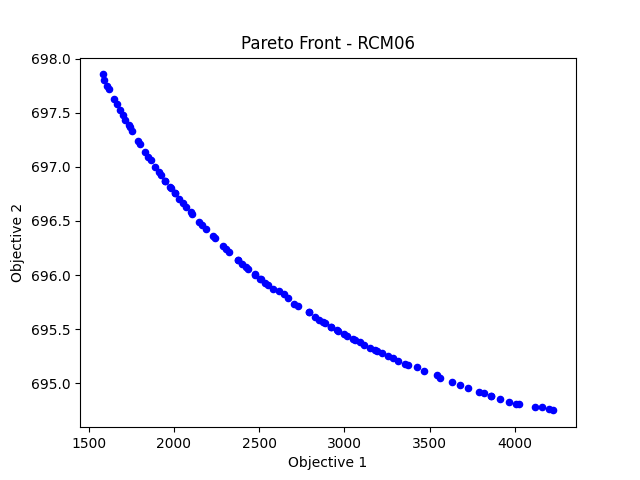
\includegraphics[width=0.8\textwidth]{results/RCM06.png}
    \caption{Frente de Pareto para o problema RCM06.}
    \label{fig:rcm06_pareto}
\end{figure}

\begin{figure}[h!]
    \centering
    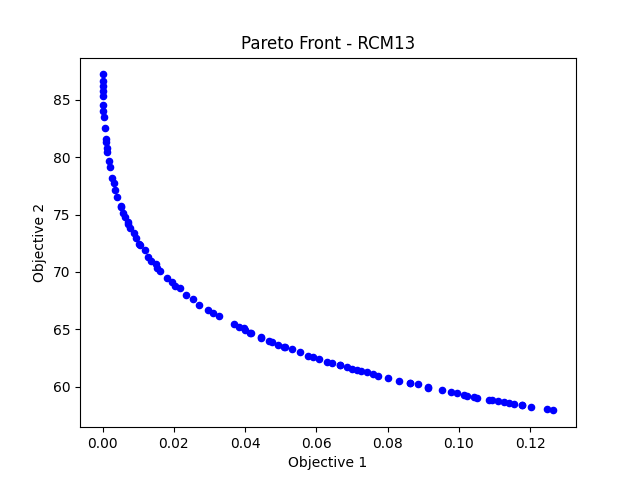
\includegraphics[width=0.8\textwidth]{results/RCM13.png}
    \caption{Frente de Pareto para o problema RCM13.}
    \label{fig:rcm13_pareto}
\end{figure}

\begin{figure}[h!]
    \centering
    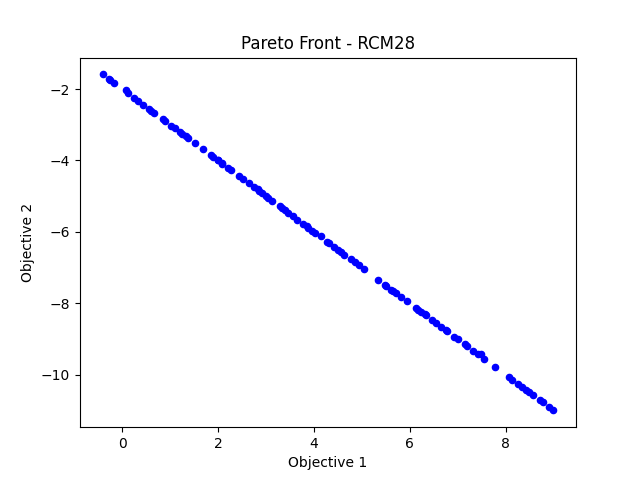
\includegraphics[width=0.8\textwidth]{results/RCM28.png}
    \caption{Frente de Pareto para o problema RCM28.}
    \label{fig:rcm28_pareto}
\end{figure}

\begin{figure}[h!]
    \centering
    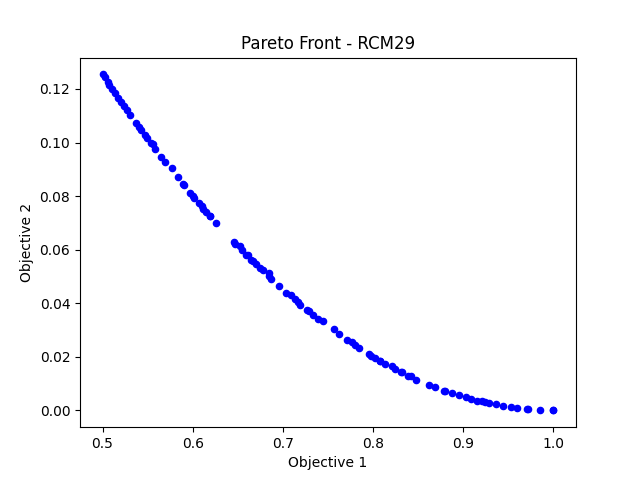
\includegraphics[width=0.8\textwidth]{results/RCM29.png}
    \caption{Frente de Pareto para o problema RCM29.}
    \label{fig:rcm29_pareto}
\end{figure}

As visualizações das frentes de Pareto confirmam a capacidade do NSGA-II em gerar um conjunto diversificado de soluções que se aproximam da verdadeira frente de Pareto. A distribuição dos pontos nos gráficos indica uma boa exploração do espaço objetivo, cobrindo uma ampla gama de compromissos entre os objetivos $f_1$ e $f_2$. A forma das frentes de Pareto varia de acordo com a natureza de cada problema, refletindo as características de suas funções objetivo e restrições.


\chapter{Discussão}
A análise dos resultados obtidos corrobora a eficácia do algoritmo NSGA-II \cite{deb2002fast, verma2021comprehensive, ma2023comprehensive} na resolução de problemas de otimização multiobjetivo, mesmo diante de cenários com variados níveis de complexidade e características. Os valores de Hipervolume, em conjunto com as visualizações das frentes de Pareto, oferecem uma base robusta para a discussão do desempenho do algoritmo.

O Hipervolume, como métrica de qualidade, demonstrou que o NSGA-II conseguiu gerar frentes de Pareto que dominam uma porção significativa do espaço objetivo. O problema RCM13, com o maior HV (1.0073), sugere que para problemas com características específicas (como as relações de produto e divisão entre variáveis), o NSGA-II pode ser particularmente eficiente em encontrar um conjunto de soluções bem distribuídas e de alta qualidade. Na prática, um HV acima de 1.0 (no espaço normalizado) indica que a frente de Pareto aproximada não apenas cobre bem o espaço objetivo, mas também pode ter soluções que superam o ponto de referência em alguns aspectos, ou que a normalização permitiu uma exploração mais ampla do que o esperado. Em um problema real de seleção de atributos, um HV elevado significaria que o algoritmo encontrou um conjunto robusto de subconjuntos de atributos, cada um oferecendo um excelente compromisso entre, por exemplo, a acurácia do modelo preditivo e a redução da dimensionalidade dos dados.

Por outro lado, o menor HV para o problema RCM28 (0.7036), que possui restrições exponenciais, indica que a complexidade e a natureza não-linear dessas restrições impactaram significativamente a capacidade do algoritmo de explorar completamente o espaço de soluções viáveis. Restrições exponenciais podem criar regiões de inviabilidade muito estreitas ou desconectadas, tornando a busca por soluções factíveis um desafio maior para o NSGA-II. Isso ressalta a importância de considerar a natureza das restrições ao selecionar e configurar algoritmos de otimização, pois elas podem limitar a diversidade e a qualidade das soluções encontradas, mesmo para algoritmos robustos como o NSGA-II.

As frentes de Pareto visualizadas graficamente confirmam a capacidade do NSGA-II em manter a diversidade das soluções. A distribuição dos pontos ao longo das curvas de Pareto é um indicativo de que o algoritmo não converge para uma única região do espaço de soluções, mas sim explora diferentes compromissos entre os objetivos. Essa diversidade é crucial em problemas de otimização multiobjetivo, pois permite que os tomadores de decisão escolham a solução que melhor se adapta às suas prioridades, mesmo que isso signifique sacrificar um objetivo em favor de outro.

É importante notar que a normalização dos objetivos para o cálculo do Hipervolume é uma etapa fundamental para garantir que a métrica não seja enviesada por diferentes escalas dos objetivos. A escolha do ponto de referência [1.1, 1.1] no espaço normalizado é uma prática comum para garantir que todas as soluções da frente de Pareto sejam consideradas na contribuição para o Hipervolume.

Em termos de aplicação prática, a capacidade do NSGA-II de gerar frentes de Pareto diversificadas é de grande valor em áreas como a seleção inteligente de atributos em bases de dados multimodais. Nesses contextos, a otimização pode envolver a minimização da dimensionalidade dos dados e a maximização da relevância dos atributos para uma tarefa específica. As soluções na frente de Pareto representariam diferentes subconjuntos de atributos, cada um com um equilíbrio distinto entre esses objetivos, permitindo que especialistas de domínio selecionem o subconjunto mais apropriado para suas necessidades. A robustez do NSGA-II, demonstrada neste estudo, o torna um candidato promissor para enfrentar os desafios da alta dimensionalidade e da heterogeneidade de dados em sistemas de inteligência artificial na indústria.


\chapter{Conclusão}
Este trabalho demonstrou a implementação e avaliação do algoritmo NSGA-II para a otimização multiobjetivo em um conjunto de problemas de teste de referência. Os resultados obtidos, tanto em termos de valores de Hipervolume quanto das frentes de Pareto aproximadas, confirmam a eficácia e a robustez do NSGA-II em encontrar soluções de compromisso para problemas com múltiplos objetivos e restrições.

A capacidade do NSGA-II de gerar frentes de Pareto diversificadas é um diferencial importante, pois oferece aos tomadores de decisão um leque de opções para escolher, permitindo um equilíbrio entre objetivos conflitantes. A análise das frentes de Pareto visualizadas graficamente reforça a boa exploração do espaço objetivo pelo algoritmo, mesmo em problemas com características complexas como o RCM28, que apresentou restrições exponenciais.

Em suma, o NSGA-II se mostrou uma ferramenta valiosa para a otimização multiobjetivo, com potencial significativo para aplicações em áreas como a seleção inteligente de atributos em bases de dados multimodais \cite{hamdani2007multi, yazdinejad2023optimized}, onde a necessidade de otimizar múltiplos critérios é constante. A metodologia empregada neste estudo, baseada na biblioteca PyMoo, provou ser eficiente para a implementação e avaliação de algoritmos de otimização.


\section*{Limitações do Trabalho}
Este trabalho, embora demonstre a eficácia do NSGA-II em problemas de otimização multiobjetivo, possui algumas limitações importantes que devem ser consideradas:
\begin{itemize}
    \item \textbf{Problemas de Teste Genéricos}: A avaliação do NSGA-II foi realizada exclusivamente em problemas de benchmark (RCM06, RCM13, RCM28, RCM29), que são genéricos e não representam diretamente a complexidade e as características específicas de bases de dados multimodais reais na indústria. Embora esses problemas sirvam para validar a robustez do algoritmo, a ausência de um estudo de caso com dados multimodais reais ou simulados limita a generalização dos resultados para o contexto prático da seleção de atributos.
    \item \textbf{Foco em um Único Algoritmo}: O estudo concentrou-se apenas no NSGA-II. Embora seja um algoritmo amplamente reconhecido e robusto, a falta de comparações diretas com outros algoritmos de otimização multiobjetivo (como SPEA2, MOEA/D, etc.) impede uma avaliação comparativa de seu desempenho em relação a outras abordagens. Isso dificulta a determinação de sua superioridade ou desvantagens em cenários específicos.
    \item \textbf{Análise Descritiva dos Resultados}: A discussão dos resultados, embora aprofundada, ainda mantém um caráter predominantemente descritivo. Uma análise mais crítica poderia explorar com maior profundidade as razões por trás de certos comportamentos do algoritmo, como o desempenho no RCM28, e traduzir o significado prático dos valores de Hipervolume em termos de problemas reais de seleção de atributos.
    \item \textbf{Ausência de Análise de Sensibilidade de Parâmetros}: Os parâmetros do NSGA-II (tamanho da população, número de gerações) foram fixados. Uma análise de sensibilidade desses parâmetros poderia fornecer insights valiosos sobre como eles afetam o desempenho do algoritmo em diferentes tipos de problemas, otimizando sua configuração para aplicações futuras.
\end{itemize}

\section{Recomendações para Trabalhos Futuros}
Para trabalhos futuros, sugere-se explorar as seguintes direções:
\begin{itemize}
    \item Investigar a aplicação do NSGA-II em problemas de seleção de atributos em bases de dados multimodais reais, avaliando seu desempenho em comparação com outras técnicas de seleção de atributos.
    \item Estudar a integração do NSGA-II com outras abordagens de otimização, como algoritmos de otimização baseados em enxame ou algoritmos de otimização de objetivo único, para melhorar a eficiência e a qualidade das soluções.
    \item Desenvolver e implementar novas métricas de avaliação para otimização multiobjetivo que sejam mais adequadas para problemas de seleção de atributos em bases de dados multimodais.
    \item Explorar a utilização de técnicas de aprendizado de máquina para auxiliar na seleção de atributos, combinando a otimização com abordagens baseadas em dados.
    \item Realizar uma análise de sensibilidade dos parâmetros do NSGA-II (e.g., tamanho da população, número de gerações, operadores genéticos) para otimizar seu desempenho em diferentes tipos de problemas.
\end{itemize}

\chapter{Outras Atividades Realizadas}
Nenhuma atividade adicional relevante foi fornecida para inclusão neste relatório.


\section*{Lições Aprendidas na Implementação com PyMoo}
A implementação do NSGA-II utilizando a biblioteca PyMoo proporcionou diversas lições valiosas, que podem ser úteis para futuros trabalhos e projetos:
\begin{itemize}
    \item \textbf{Facilidade de Uso da PyMoo}: A biblioteca PyMoo se mostrou extremamente intuitiva e poderosa para a definição de problemas de otimização multiobjetivo e a aplicação de algoritmos. A estrutura de classes para `Problem`, `Algorithm` e `Minimize` simplifica significativamente o processo de codificação, permitindo que o foco seja mantido na lógica do problema e na análise dos resultados, em vez de detalhes de implementação de baixo nível.
    \item \textbf{Visualização Integrada}: A capacidade de gerar visualizações das frentes de Pareto diretamente a partir dos resultados do `minimize` é um recurso valioso para a análise qualitativa do desempenho do algoritmo. Isso agiliza a compreensão da distribuição e diversidade das soluções encontradas.
    \item \textbf{Métricas de Avaliação Prontas para Uso}: A PyMoo oferece implementações prontas de métricas de avaliação como o Hipervolume, o que facilita a quantificação da qualidade das frentes de Pareto. A normalização dos objetivos é um passo crucial para o uso correto dessas métricas, e a biblioteca oferece as ferramentas necessárias para isso.
    \item \textbf{Reprodutibilidade}: A possibilidade de fixar a semente do gerador de números aleatórios (`seed`) é fundamental para garantir a reprodutibilidade dos experimentos, um aspecto crítico em pesquisa científica e engenharia.
    \item \textbf{Desafios com Restrições Complexas}: Embora a PyMoo simplifique a definição de restrições, a complexidade intrínseca de algumas restrições (como as exponenciais no RCM28) ainda representa um desafio para o algoritmo. A análise do impacto dessas restrições no desempenho do NSGA-II reforça a necessidade de uma compreensão aprofundada do problema antes da aplicação de qualquer algoritmo de otimização.
\end{itemize}

\bibliographystyle{abntex2-alf}
\bibliography{referencias}

\appendix
\chapter{Anexo - Códigos Python}

Este anexo contém os códigos Python utilizados para a implementação dos problemas de teste e a execução do algoritmo NSGA-II. Os arquivos são:

\begin{itemize}
    \item \texttt{problems/rcm06.py}: Implementação do problema de teste RCM06.
    \item \texttt{problems/rcm13.py}: Implementação do problema de teste RCM13.
    \item \texttt{problems/rcm28.py}: Implementação do problema de teste RCM28.
    \item \texttt{problems/rcm29.py}: Implementação do problema de teste RCM29.
    \item \texttt{evaluate.py}: Script principal para executar os problemas, aplicar o NSGA-II, calcular o Hipervolume e gerar os gráficos das frentes de Pareto.
\end{itemize}

Os códigos estão disponíveis no diretório do projeto e podem ser consultados para detalhes de implementação.


\end{document}
